\section{EMMC} eMMC stands for embedded MultiMedia Card and refers to a package consisting of both flash memory and a flash memory controller. The controller here is divided into 2 parts: 1. Host controller 2. Device controller. Host controller sits on the host device and is usually operates on a higher layer of programming. Device controller sits inside the flash memory hardware. It takes signals controlled by the Host controller and converts them into interpretable signals for the flash memory. The eMMC specification covers the behavior of the interface and the device controller. As part of this specification the existence of a host controller and a memory storage array are implied but the operation of these pieces is not fully specified.

\subsection{eMMC Device Overview}
The eMMC device transfers data via a configurable number of data bus signals. The communication signals are:

\begin{itemize}
  \item \textbf{CLK} Each cycle of this signal directs a one bit transfer on the command and either a one bit (1x) or a two bits transfer (2x) on all the data lines. The frequency may vary between zero and the maximum clock frequency.

  \item \textbf{Data Strobe} This signal is generated by the device and used for data output and CRC status response output in HS400 mode. The frequency of this signal follows the frequency of CLK. For data output each cycle of this signal directs two bits transfer(2x) on the data one bit for positive edge and the other bit for negative edge. For CRC status response output, the CRC status is latched on the positive edge only, and don't care on the negative edge.

  \item \textbf{CMD} This signal is a bidirectional command channel used for device initialization and transfer of commands. The CMD signal has two operation modes: opendrain for initialization mode, and push\textendash pull for fast command transfer. Commands are sent from the eMMC host controller to the eMMC device and responses are sent from the device to the host.

  \item \textbf{DAT0\textendash DAT7} These are bidirectional data channels. The DAT signals operate in push\textendash pull mode. Only the device or the host is driving these signals at a time. By default, after power up or reset, only DAT0 is used for data transfer. A wider data bus can be configured for data transfer, using either DAT0\textendash DAT3 or DAT0\textendash DAT7, by the eMMC host controller. The eMMC device includes internal pull\textendash ups for data lines DAT1\textendash DAT7. Immediately after entering the 4\textendash bit mode, the device disconnects the internal pull ups of lines DAT1, DAT2, and DAT3. Correspondingly, immediately after entering to the 8\textendash bit mode the device disconnects the internal pull\textendash ups of lines DAT1\textendash DAT7.
\end{itemize}

All communication between host and device are controlled by the host (master). The host sends a command, which results in a device response. Five operation modes are defined for the eMMC system (hosts and devices):

\begin{itemize}
  \item {Boot mode} The device will be in boot mode after power cycle, reception of CMD0 with argument of 0xF0F0F0F0 or the assertion of hardware reset signal.

  \item {Device identification mode} The device will be in device identification mode after boot operation mode is finished or if host and /or device does not support boot operation mode. The device will be in this mode, until the SET\_RCA command (CMD3) is received.

  \item {Interrupt mode} Host and device enter and exit interrupt mode simultaneously. In interrupt mode there is no data transfer. The only message allowed is an interrupt service request from the device or the host.

  \item {Data transfer mode} The device will enter data transfer mode once an RCA is assigned to it. The host will enter data transfer mode after identifying the device on the bus.

  \item {Inactive mode} The device will enter inactive mode if either the device operating voltage range or access mode is not valid. The device can also enter inactive mode with GO\_INACTIVE\_STATE command (CMD15). The device will reset to Pre-idle state with power cycle.
\end{itemize}

\begin{figure}[H]
\begin{center}
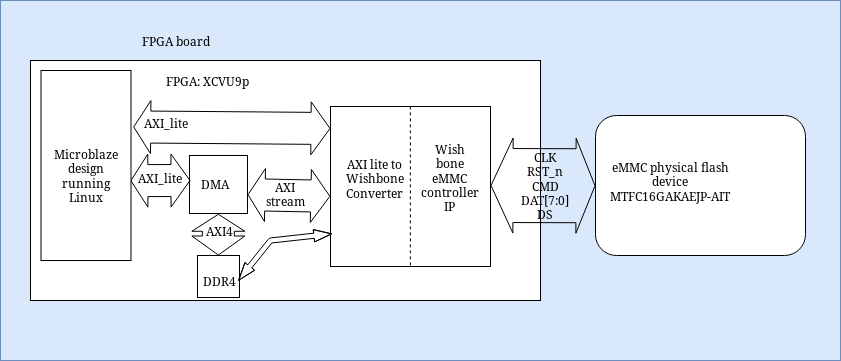
\includegraphics[width=\textwidth]{images/emmc.png}
\caption{Internal block diagram of EMMC IP}
\label{emmc}
\end{center}
\end{figure}
If the CMD line is held LOW for 74 clock cycles and more after powerup or reset operation (either through CMD0 with the argument of 0xF0F0F0F0 or assertion of hardware reset for eMMC, if it is enabled in Extended CSD register byte [162], bits [1:0]) before the first command is issued, the slave recognizes that boot mode is being initiated and starts preparing boot data internally. Timing diagram of EMMC IP Boot up sequence is shown in \figref{BootUpSeqTiming}

\begin{figure}[H]
\begin{center}
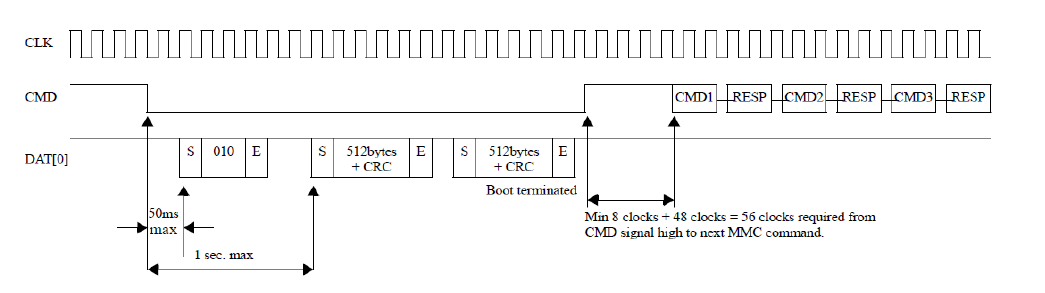
\includegraphics[width=\textwidth]{images/BootUpSeqTiming.png}
\caption{Timing diagram of EMMC IP Boot up sequence}
\label{BootUpSeqTiming}
\end{center}
\end{figure}

The partition from which the master will read the boot data can be selected in advance using EXT\_CSD byte [179], bits [5:3]. The data size that the master can read during boot operation can be calculated as 128KB X BOOT\_SIZE\_MULT (EXT\_CSD byte [226]). Within 1 second after the CMD line goes LOW, the slave starts to send the first boot data to the master on the DAT line(s). The master must keep the CMD line LOW to read all of the boot data. The master must use push-pull mode until boot operation is terminated.

The master can choose to use single data rate mode with backward-compatible interface timing, single data rate with high-speed interface timing or dual data rate timing (if it supported) shown in 10.6 by setting a proper value in EXT\_CSD register byte [177] bits [4:3]. EXT\_CSD register byte [228], bit 2 tells the master if the high-speed timing during boot is supported by the device. The master can also choose to use the dual data rate mode with interface during boot by setting '10' in EXT\_CSD register byte [177], bits [4:3]. EXT\_CSD register byte [228], bit 1 tells the master if the dual data rate mode during boot is supported by the device.

The master can choose to receive boot acknowledge from the slave by setting '1' in EXT\_CSD register, byte [179], bit 6, so that the master can recognize that the slave is operating in boot mode. If boot acknowledge is enabled, the slave has to send acknowledge pattern '010' to the master within 50ms after the CMD line goes LOW. If boot acknowledge is disabled, the slave will not send out acknowledge pattern '0-1-0.' In the single data rate mode, data is clocked out by the device and sampled by the host with the rising edge of the clock and there is a single CRC per data line.

In the dual data rate mode, data is clocked out with both the rising edge of the clock and the falling edge of the clock and there are two CRC appended per data line. In this mode, the block length is always 512 bytes, and bytes come interleaved in either 4-bit or 8-bit width configuration. Bytes with odd number (1,3,5, ... ,511) shall be sampled on the rising edge of the clock by the host and bytes with even number (2,4,6, ... ,512) shall be sampled on the falling edge of the clock by the host. The device will append two CRC16 per each valid data line, one corresponding to the bits of the 256 odd bytes to be sampled on the rising edge of the clock by the host and the second for the remaining bits of the 256 even bytes of the
block to be sampled on the falling edge of the clock by the host. All timings on DAT lines shall follow DDR timing mode. The start bit, the end bit and Boot acknowledge bits are only valid on the rising edge of the clock. The value of the falling edge is not guaranteed. The master can terminate boot mode with the CMD line HIGH. If the master pulls the CMD line HIGH in the middle of data transfer, the slave has to terminate the data transfer or acknowledge pattern within NST clock cycles (one data cycle and end bit cycle). If the master terminates boot mode between consecutive blocks, the slave must release the data line(s) within NST clock cycles.

Boot operation will be terminated when all contents of the enabled boot data are sent to the master. After boot operation is executed, the slave shall be ready for CMD1 operation and the master needs to start a normal MMC initialization sequence by sending CMD1. Please find the boot sequence in \figref{BootUpSeq} which will be operated by the eMMC driver in the hindsight for initialization and then for the operation of the eMMC memory.

\begin{figure}[H]
\begin{center}
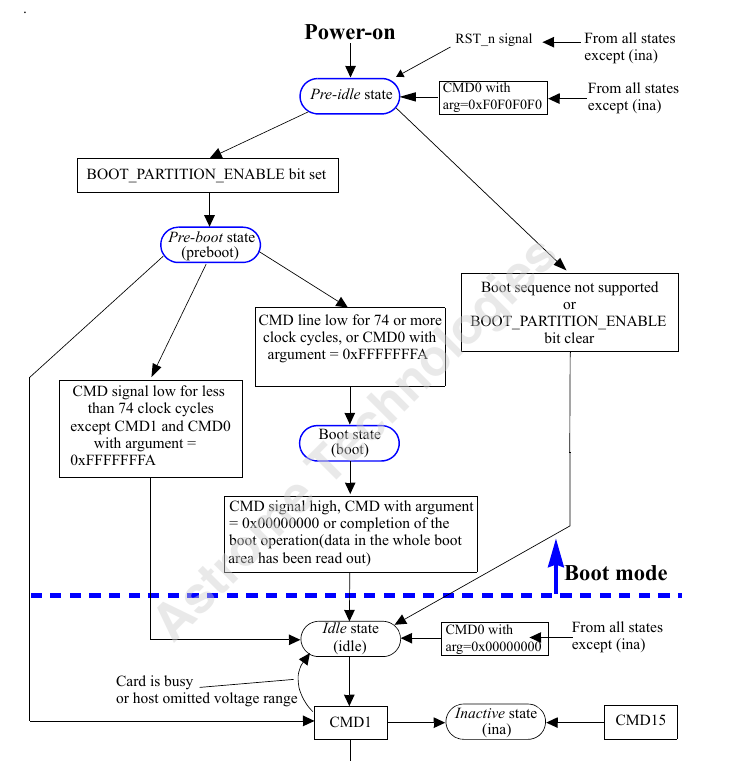
\includegraphics[width=\textwidth]{images/BootUpSeq.png}
\caption{EMMC IP Boot up sequence}
\label{BootUpSeq}
\end{center}
\end{figure}


\pagebreak
 
